\documentclass{ximera}

\graphicspath{{./}{./graphics/}{./content/01_4_cylindrical_coords/graphics/}}

\title{Cylindrical Coordinates}
\author{Melissa Lynn}
\outcome{Understand the geometry of cylindrical coordinates. Be able to describe curves, surfaces, and regions using cylindrical coordinates, and convert between cylindrical and Cartesian coordinates.}

\begin{document}
\begin{abstract}
\end{abstract}
\maketitle

We've seen how points in $\mathbb{R}^2$ can be written using polar coordinates, and we've seen how polar coordinates can be useful for describing some shapes that are difficult to describe in Cartesian coordinates.

We'd now like to extend this idea to $\mathbb{R}^3$, using a coordinate system called \emph{cylindrical coordinates}. Like polar coordinates, cylindrical coordinates will be useful for describing shapes in $\mathbb{R}^3$ that are difficult to describe using Cartesian coordinates. Later in the course, we will also see how cylindrical coordinates can be useful in calculus, when evaluating limits or integrating in Cartesian coordinates is very difficult.

\section*{Cylindrical coordinates}

Cylindrical coordinates are really just an extension of polar coordinates. For points in the $xy$-plane, we describe them using $r$ and $\theta$, where $r$ is the distance from the origin and $\theta$ is the angle with the positive $x$-axis. We then append a $z$-coordinate, which tells us the vertical displacement of the point.

In other words, for a point $(x,y,z)$ given in Cartesian coordinates, we consider its projection onto the $xy$-plane, which gives us the point $(x,y)$ in $\mathbb{R}^2$. We find the polar coordinates $(r,\theta)$ of the point $(x,y)$, and then we write our original point $(x,y,z)$ in cylindrical coordinates as $(r,\theta, z)$.

\begin{image}
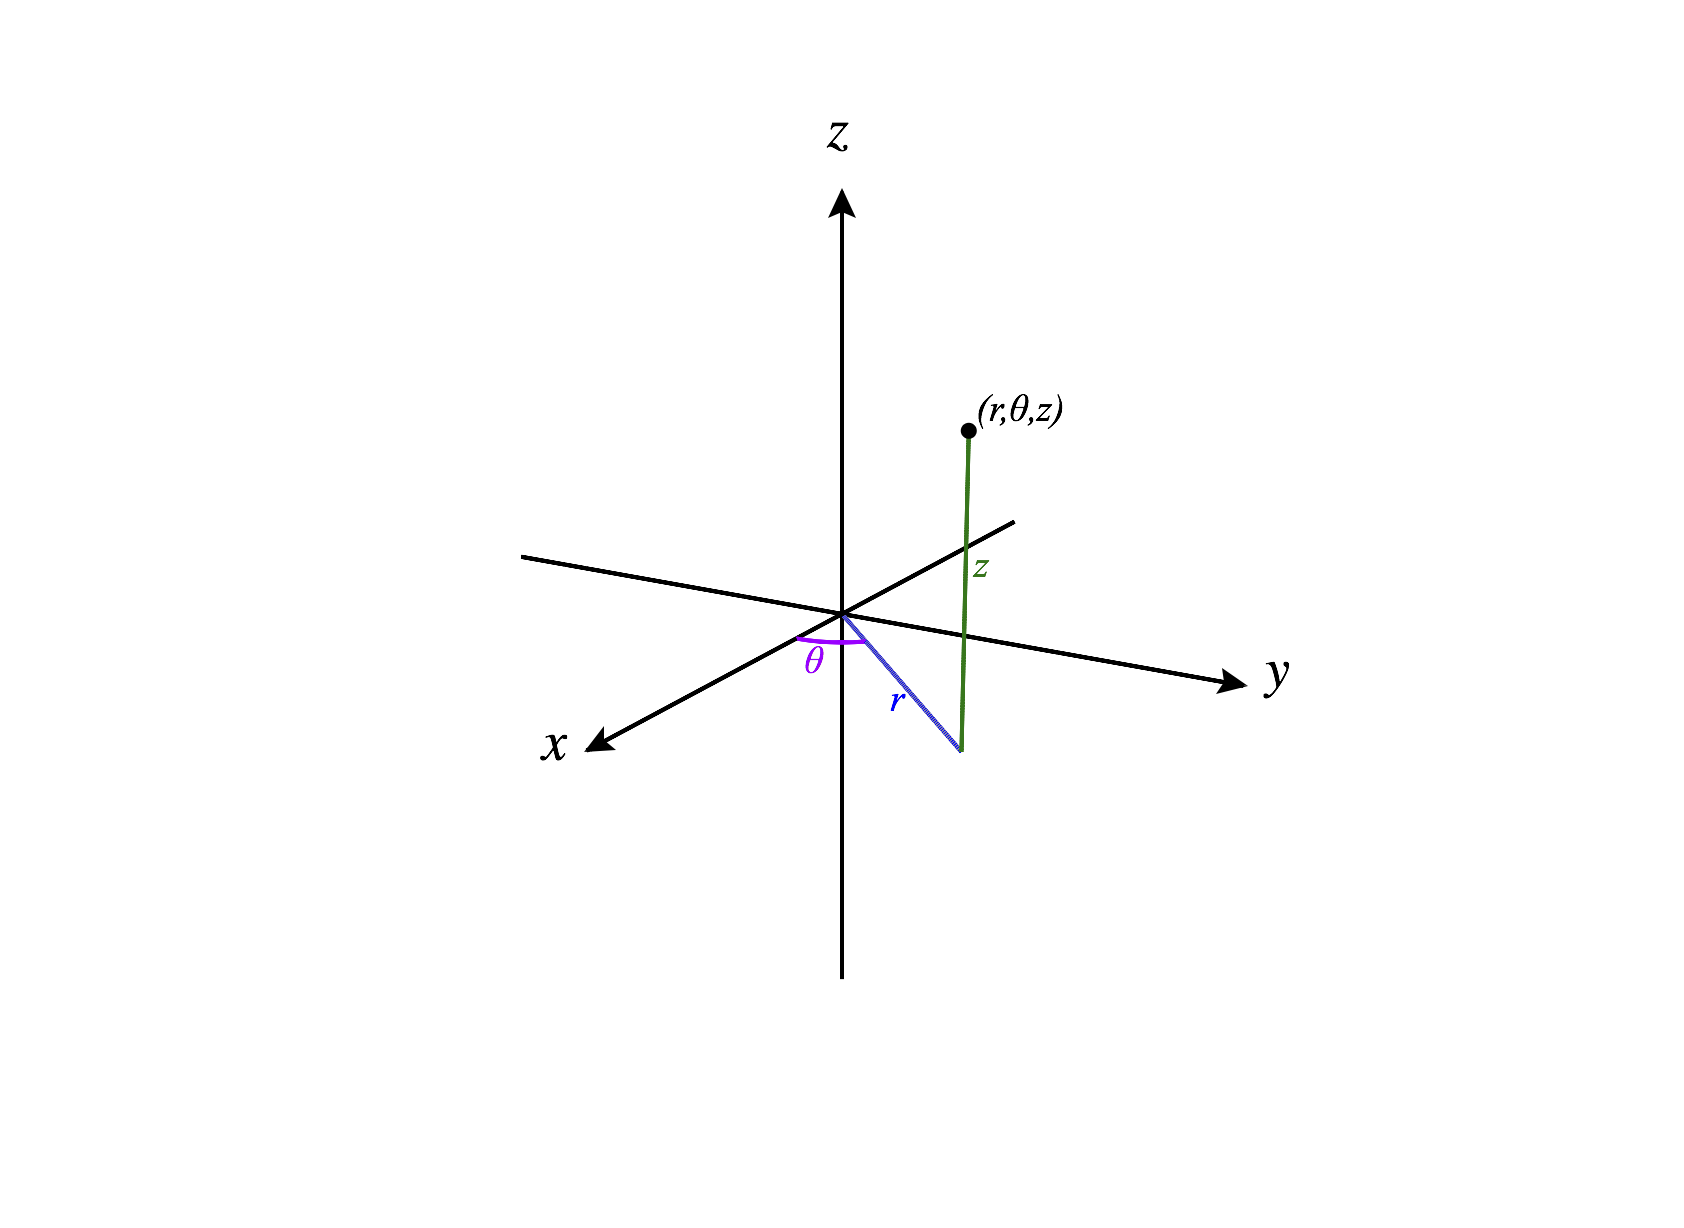
\includegraphics[width = \textwidth]{CalcPlot3D-cylindrical}
\end{image}

\begin{example}
We'll convert the point $(x,y,z) = (1,1,1)$ to cylindrical coordinates.

We can figure out $r$ and $\theta$ by projecting our point onto the $xy$-plane, giving us the point $(1,1)$ in $\mathbb{R}^2$. Then we represent $(1,1)$ in polar coordinates, so we have
\[
(r,\theta) = \answer{(\sqrt{2}, \pi/4)}.
\]
For last coordinate, $z$, notice that this is telling us the height of the point, which is the exact same as the $z$-coordinate of the point written in Cartesian coordinates! So, our $z$ coordinate is $\answer{1}$, and the point $(x,y,z) = (1,1,1)$ can be written in cylinderical coordinates as
\[
(r,\theta,z) = \answer{(\sqrt{2}, \pi/4, 1)}.
\]
\end{example}

You may use this \href{https://mathinsight.org/cylindrical_coordinates}{applet} to experiment with how changing the different coordinates changes the point given in cylindrical coordinates.

\section*{Uniqueness}

When we studied polar coordinates, we saw that there were many different ways to represent a point. For example, the point $(x,y) = (0,1)$ could be written as $(r,\theta) = (1,\pi/2)$, $(1,5\pi/2)$, or even $(-1,3\pi/2)$. And the origin was especially devious, it could be written as $(0,\theta)$ for any angle $\theta$.

Because of this and the relationship between polar and cylindrical coordinates, it's not surprisingly that cylindrical coordinates have similar issues with uniqueness. For example, the point $(0,1,1)$ can be written as $(r,\theta, z) = (1,\pi/2,1)$, $(1,5\pi/2,1)$, $(-1, 3\pi/w, 1)$, and so on. Any point on the $z$-axis can be written as $(0,\theta,z)$, where $z$ is its $z$-coordinate, and $\theta$ is any angle.

\begin{problem}
Which of the following, written in cylindrical coordinates, is equivalent to the point $(x,y,z) = (1,1,1)$? Select all that apply.
\begin{selectAll}
\choice{$(1,1,1)$}
\choice{$(1,\pi/4, 1)$}
\choice[correct]{$\sqrt{2},\pi/4, 1)$}
\choice{$(-1,3\pi/4, 1)$}
\choice{$-\sqrt{2},\pi/4,1)$}
\choice[correct]{$-\sqrt{2}, -3\pi/4,1)$}
\end{selectAll}
\end{problem}

As with polar coordinates, in situations where uniqueness is important, we will often make the restrictions $r\geq 0$ and $0\leq\theta<2\pi$. Unfortunately, this restriction does not completely eliminate the issues with uniqueness, as there are still infinitely ways to describe the origin.

\section*{Constant-coordinate surfaces}

Let's look at what happens in cylindrical coordinates when we set each of the coordinates $r,\theta,z$ to be constant, with the standard restrictions that $0\leq r$ and $0\leq \theta\leq \pi/2$. This can give us insight to how cylindrical coordinates behave.

We'll begin by examining the set of points $(r,\theta, z)$, where $r=C$ is a constant. We have that $r=C$ is constant, which means that the distance between any such point and the $z$ axis is constant, $C$. Also, $\theta$ and $z$ can be anything. This will give us the cylinder of radius $C$, centered at the $z$-axis.

\begin{image}
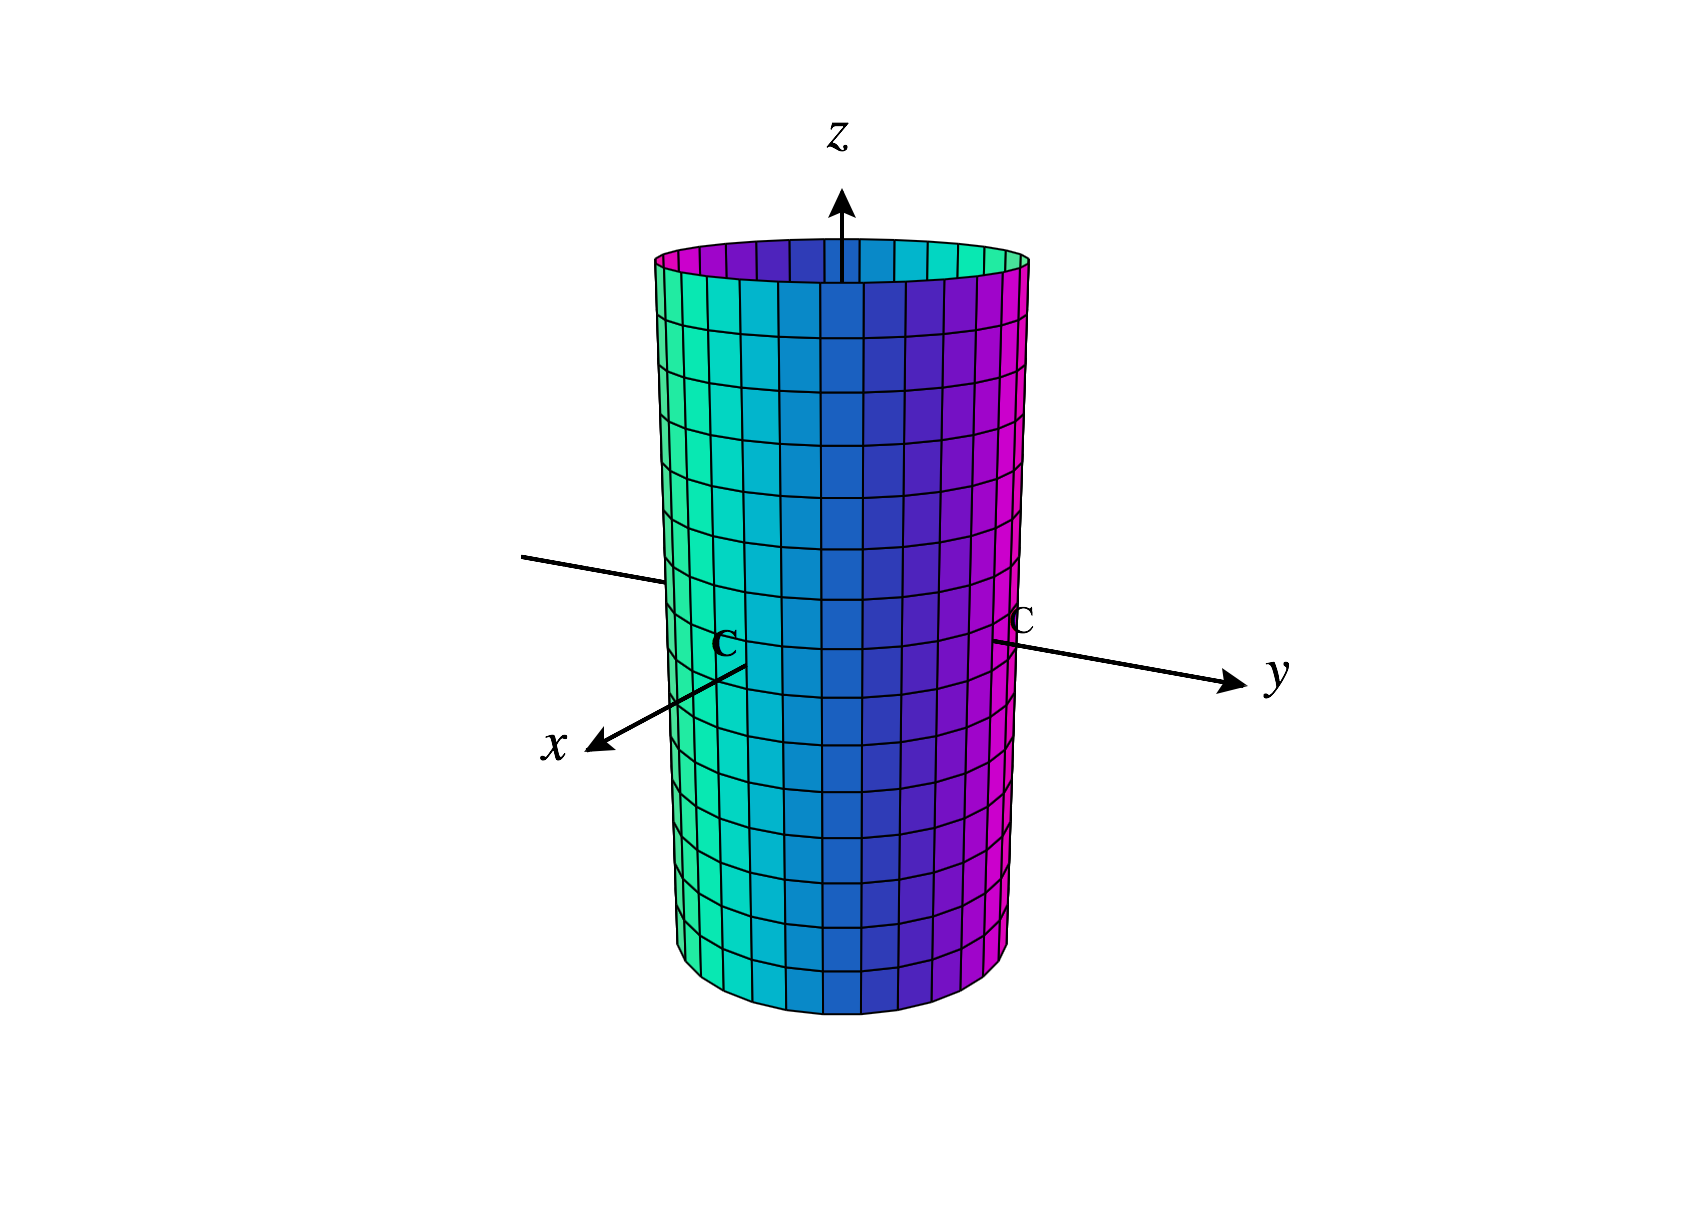
\includegraphics[width=\textwidth]{CalcPlot3D-r_constant}
\end{image}

Next, we'll investigate the set of points $(r,\theta,z)$, where $\theta = C$ is constant. Let's consider the projection of this point onto the $xy$-plane. The projection will make an angle $C$ with the positive $x$-axis, and have distance $r\geq 0$ from the origin. The height of the point can be any real number. From these observations, we conclude that the set of such points is the following half plane in $\mathbb{R}^3$.

\begin{image}
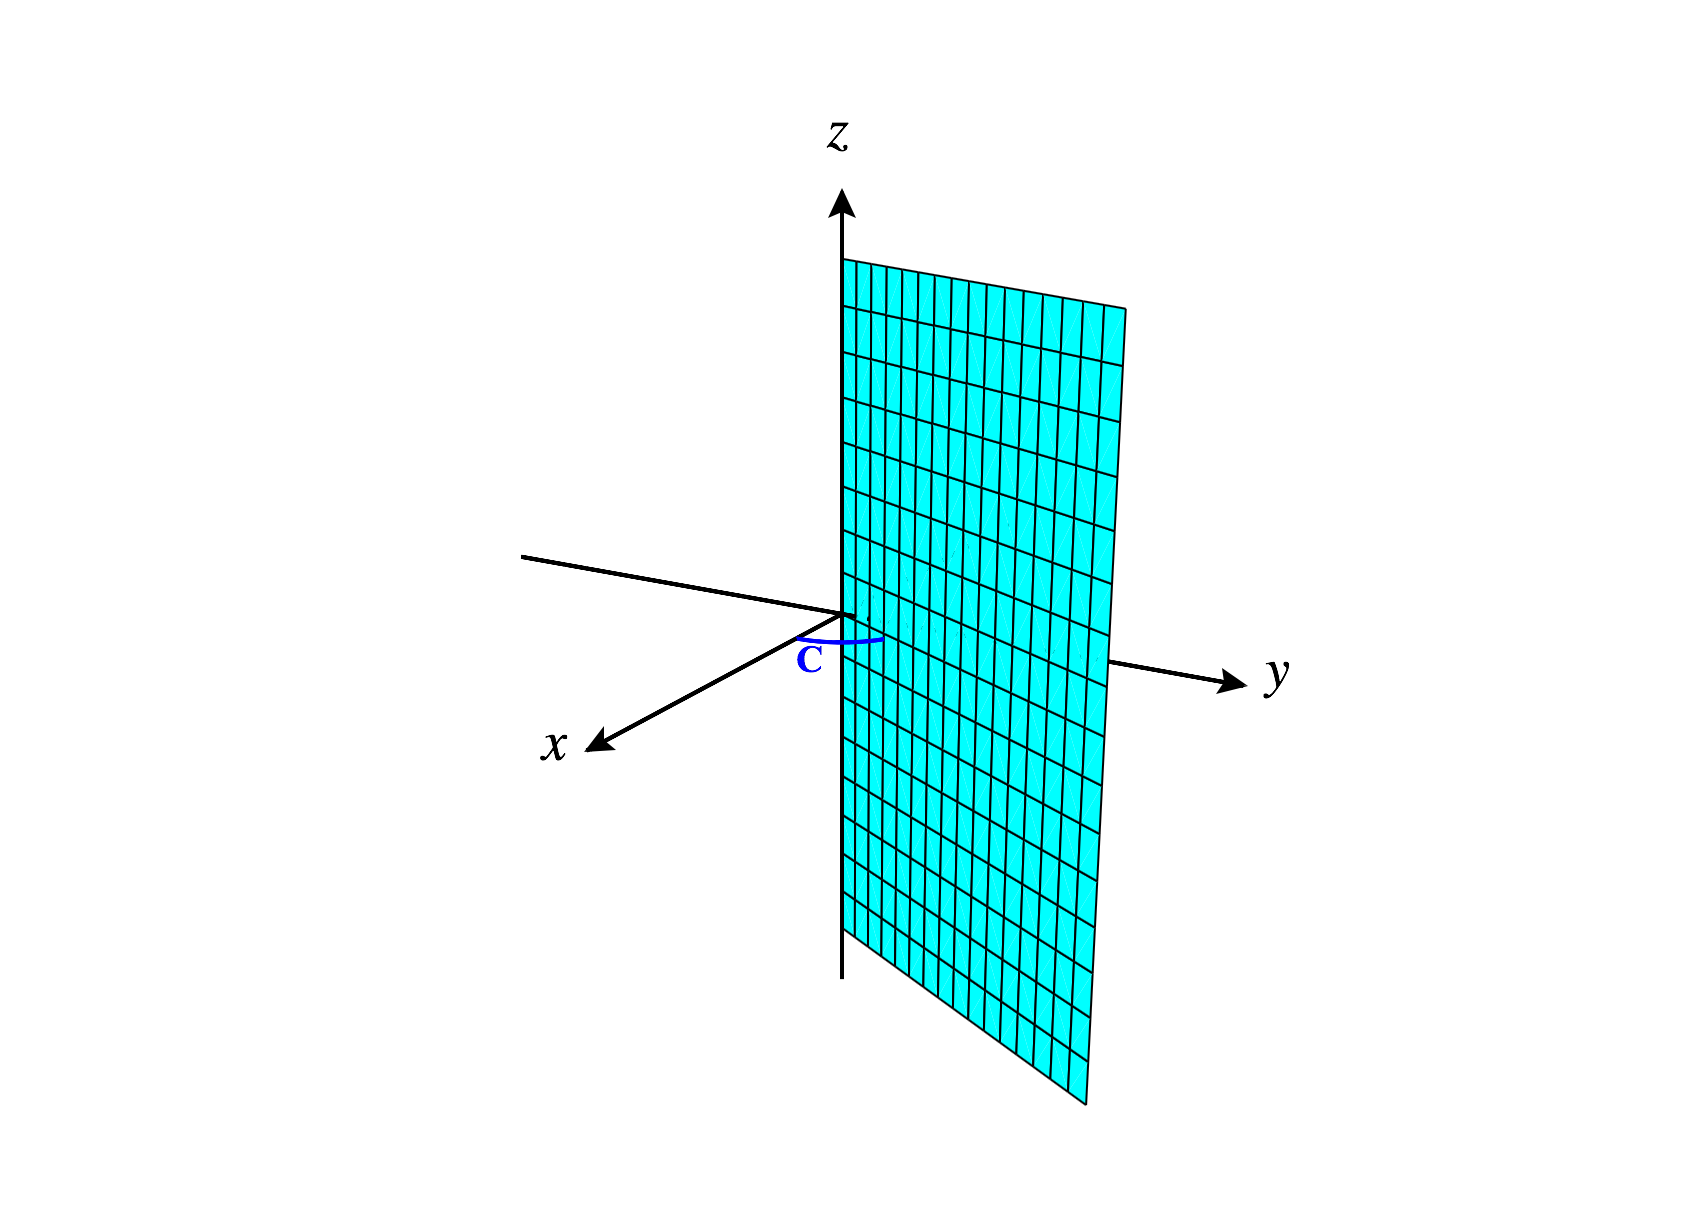
\includegraphics[width=\textwidth]{CalcPlot3D-theta_constant}
\end{image}

Note that if we didn't have the restriction $r\geq 0$, we would get an entire plane rather than a half plane.

Finally, we'll consider the set of points $(r,\theta, z)$, where $z = C$ is constant. Since $z = C$, we will only have points at height $C$. Varying $r$ and $\theta$ will then give us all points in the plane at height $C$ parallel to the $xy$-plane, as below.

\begin{image}
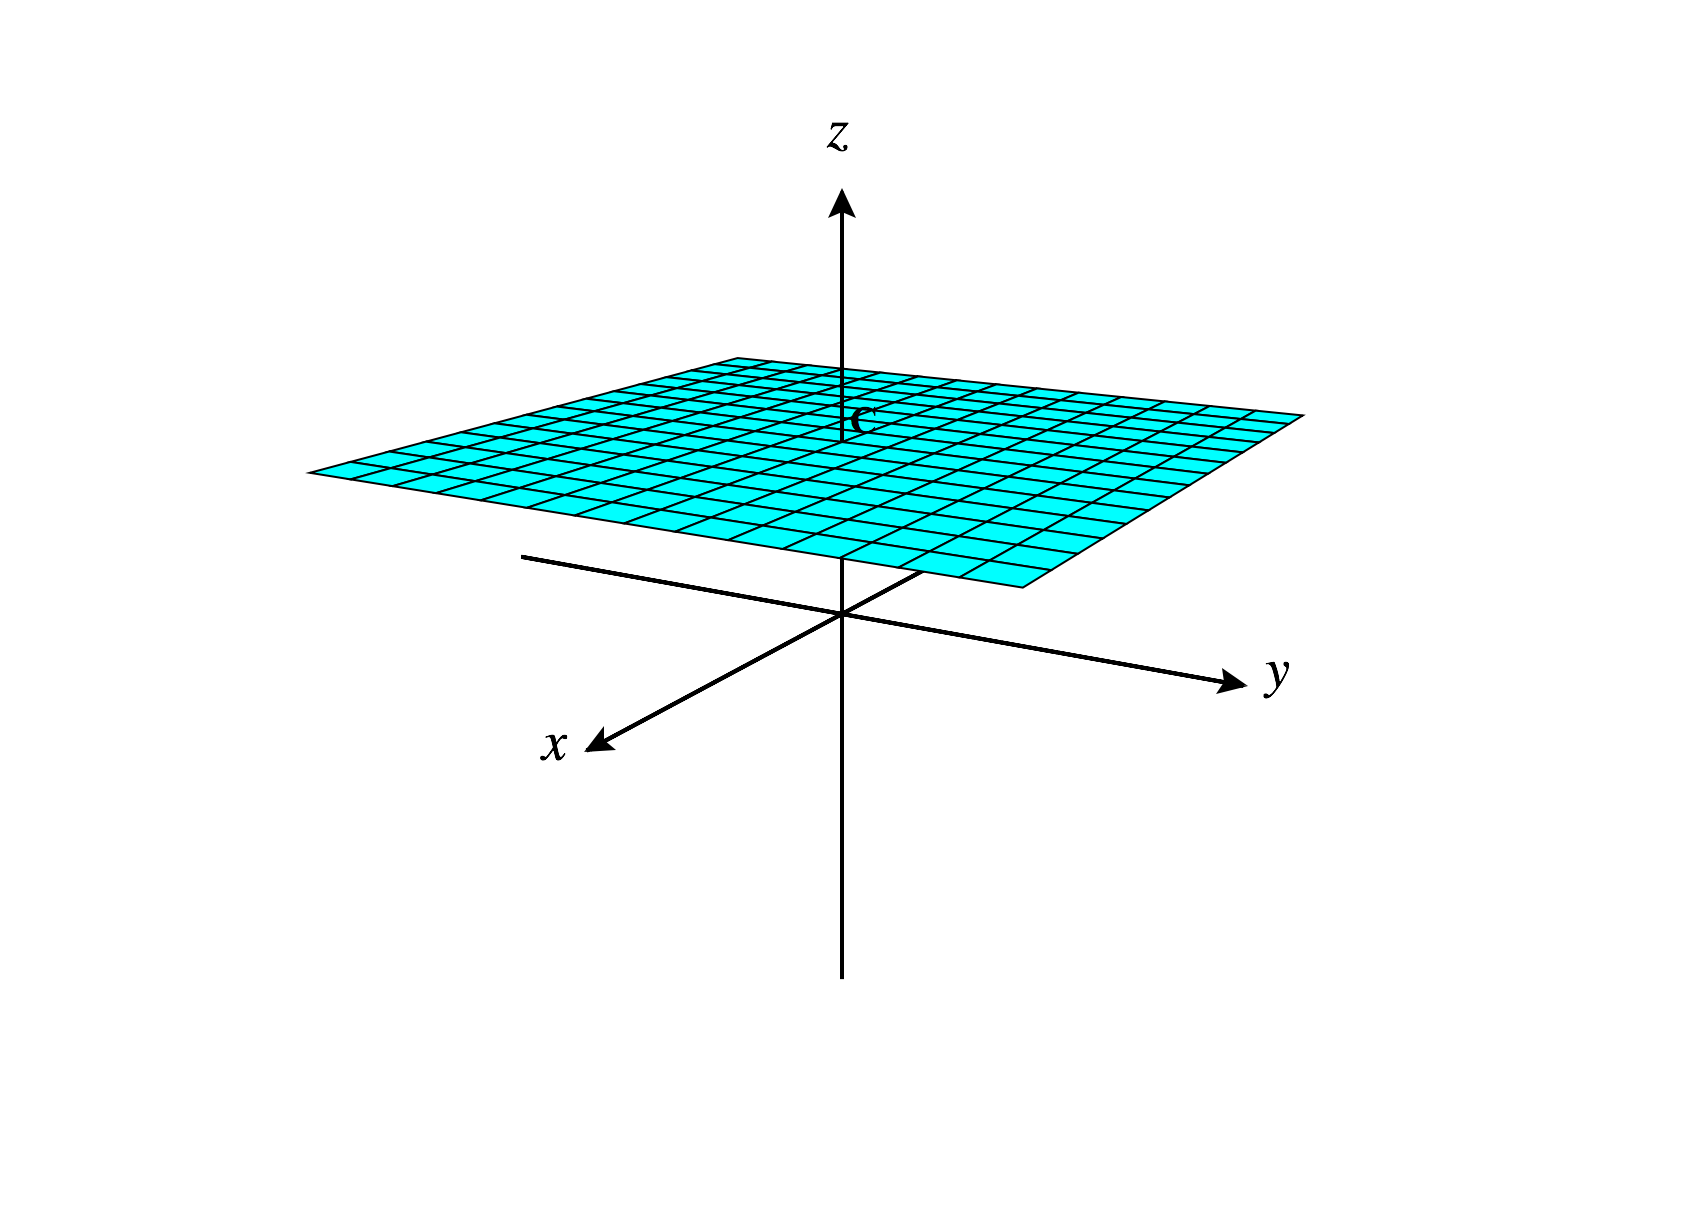
\includegraphics[width=\textwidth]{CalcPlot3D-z_constant}
\end{image}

\section*{Converting between Cartesian and cylindrical coordinates}

Perhaps not surprisingly, converting between Cartesian coordinates and cylindrical coordinates is very similar to how we converted between Cartesian coordinates and polar coordinates. That is, we can use the equations:
\begin{align*}
x &= r\cos\theta, \\
y &= r\sin\theta, \\
z &= z,\\
r^2 &= x^2 + y^2, \\
\tan\theta &= \frac{y}{x}.
\end{align*}


\begin{example}
We'll convert $z = \sqrt{1-r^2}$ to Cartesian coordinates.

Using $r^2 = x^2 + y^2$, we have
\[
z = \sqrt{1-x^2-y^2}.
\]
You may recognize this as the top half of the sphere of radius $1$ centered at the origin. You could also rewrite this as
\[
x^2+y^2+z^2=1,
\]
keeping in mind that $z\geq 0$.

\begin{image}

\includegraphics[width=\textwidth]{CalcPlot3D-half_sphere}
\end{image}

\end{example}

\begin{example}
Consider the surface in $\mathbb{R}^3$ described by the equation $(x-2)^2 + y^2 = 1$. Note that $z$ has no restrictions. This surface is the cylinder of radius $1$ centered at the vertical line through the point $(1,0,0)$.

\begin{image}
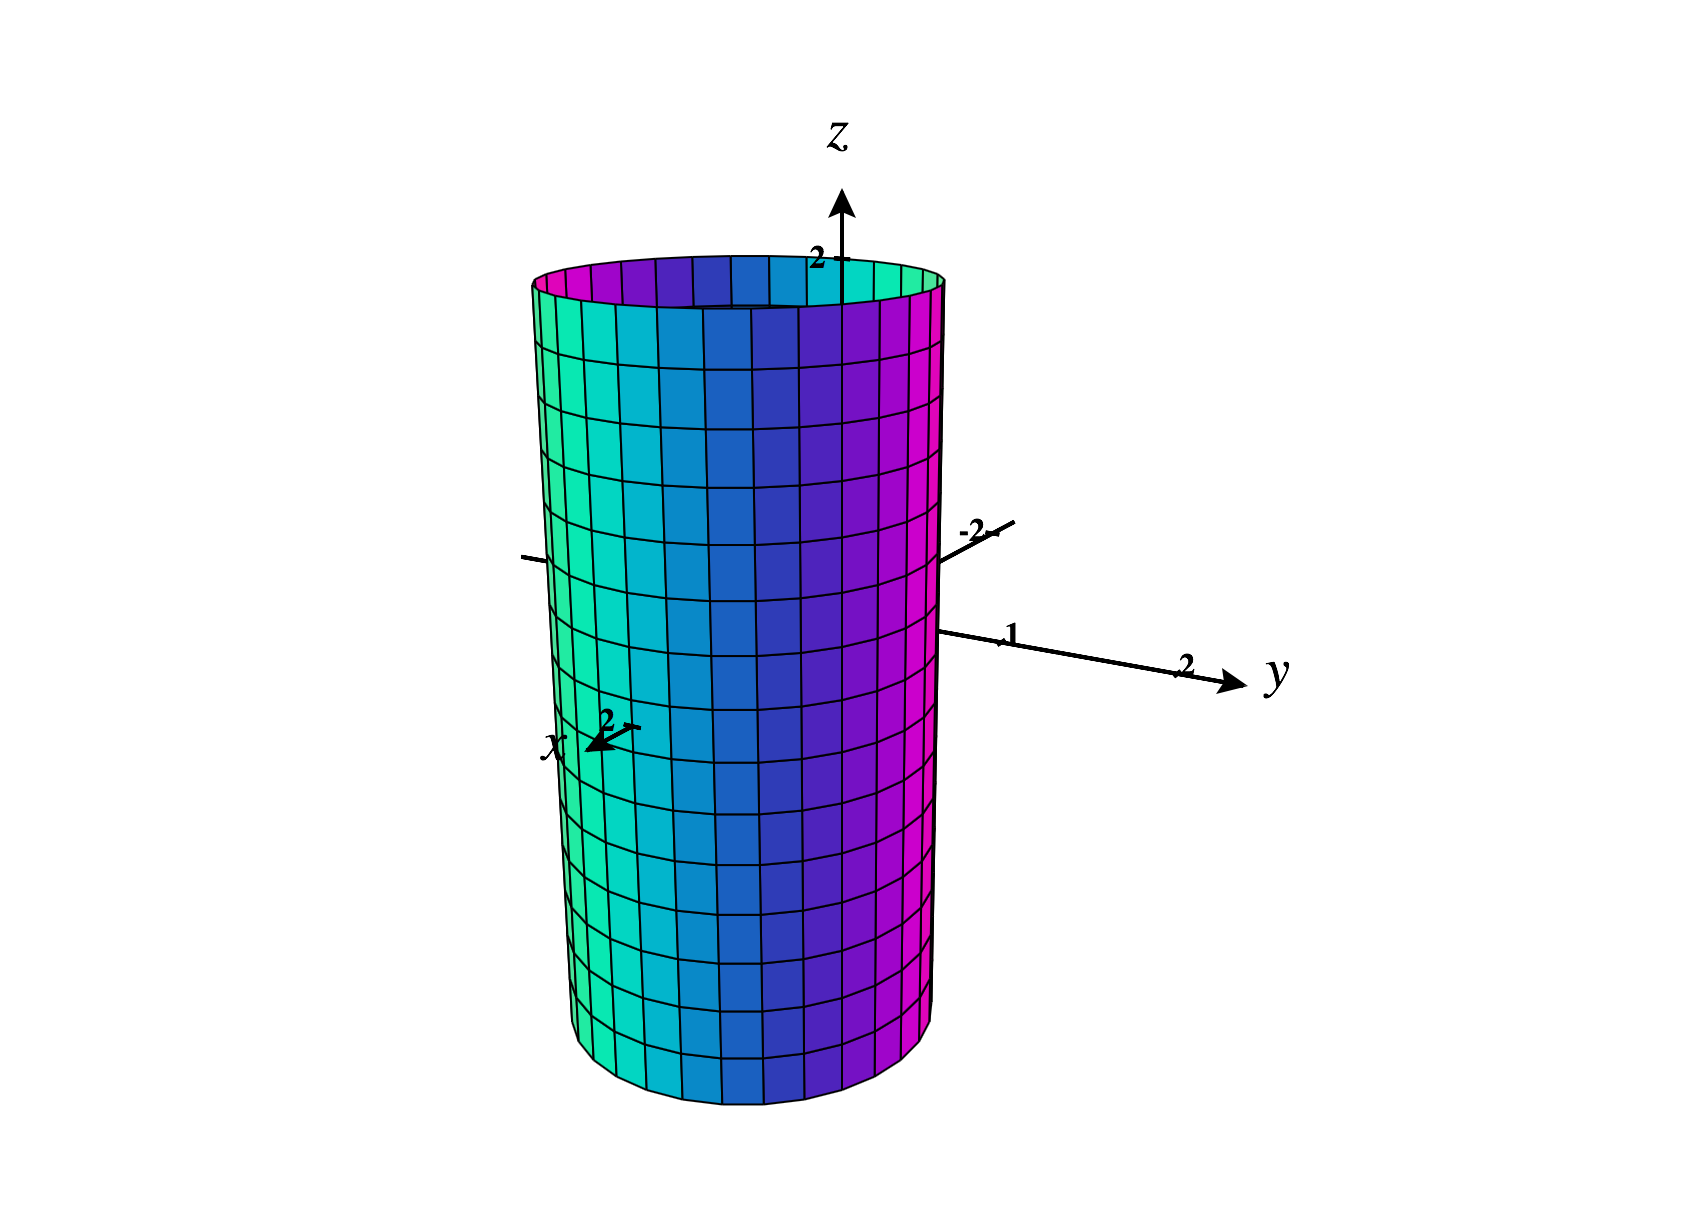
\includegraphics[width=\textwidth]{CalcPlot3D-cylinder_100}
\end{image}

We'll determine how to describe this cylinder in cylindrical coordinates, by converting the equation to cylindrical coordinates.

Expanding the expression, we have
\[
x^2-4x+1+y^2 =1.
\]
Substituting $r^2 = x^2+y^2$ and subtracting $1$ from each side, we obtain
\[
r^2-4x=0.
\]
We then substitute $x = r\cos\theta$.
\[
r^2-4r\cos\theta = 0.
\]
Dividing both sides by $r$, we have
\[
r-4\cos\theta = 0,
\]
or
\[
r = 4\cos\theta,
\]
and $z$ can be anything.

When we divided by $r$, we implicitly assumed that $r$ was not $0$. This means that we might accidentally be omitting the origin, but if we take $\theta = \pi/2$, we have
\[
r = 4\cos(0) = 0,
\]
so the origin is already included in the surface $r = 4\cos\theta$.

\end{example}

\begin{problem}
For each of the following equations in cylindrical coordinates, select the type of shape they define.

$r = \cos\theta$
\begin{multipleChoice}
\choice{plane}
\choice[correct]{cylinder}
\choice{sphere}
\choice{other}
\end{multipleChoice}

$z = r\cos\theta$
\begin{multipleChoice}
\choice[correct]{plane}
\choice{cylinder}
\choice{sphere}
\choice{other}
\end{multipleChoice}

$z = -r$
\begin{multipleChoice}
\choice{plane}
\choice{cylinder}
\choice{sphere}
\choice[correct]{other}
\end{multipleChoice}
\end{problem}


\textit{Images were generated using \href{https://www.monroecc.edu/faculty/paulseeburger/calcnsf/CalcPlot3D/}{CalcPlot3D}.}

\end{document}